\documentclass[11pt, letterpaper]{article}
\usepackage[a4paper, total={7in, 9in}]{geometry}
% Including and changing fonts %
\usepackage[T1]{fontenc}
\usepackage{cmbright}
\usepackage{DejaVuSansMono}
\setlength{\parindent}{0pt}
\usepackage[dvipsnames]{xcolor}
\usepackage{soul}
\usepackage{color}


\usepackage{atbegshi}
\usepackage{graphicx}
% For coloring within verbatims %
\usepackage{fancyvrb}
\usepackage{listings}
\lstset{%
        basicstyle=\ttfamily,
        breaklines=true,
        columns=fullflexible,
        escapeinside = ||,
        breakindent=0pt}
% Add capability to frame code with a colored rectangle
\usepackage[framemethod=tikz]{mdframed}
\lstnewenvironment{code}{}{}

% My custom colors %
\definecolor{punctuationColor}{RGB}{105, 152, 171}
\definecolor{codeBackgroundColor}{RGB}{26, 55, 77}
\definecolor{trueBoolColor}{RGB}{177,208,224}
\definecolor{variableNameColor}{RGB}{78, 159, 61}
\definecolor{classNameColor}{RGB}{183,66,60}
\definecolor{objectNameColor}{RGB}{222,131,77}
\definecolor{stringColor}{RGB}{240, 210, 144}
\definecolor{arrayNameColor}{RGB}{216, 233, 168}

\DeclareRobustCommand{\hlbackground}[1]{{\sethlcolor{codeBackgroundColor}\hl{#1}}}
\DeclareRobustCommand{\colorobject}[1]{{\color{objectNameColor}{#1}}}


\graphicspath{ {./images/} }
% For centering verbatims %
\usepackage{fancyvrb}
%  Remove pesky error-prone first page %
\AtBeginDocument{\AtBeginShipoutNext{\AtBeginShipoutDiscard}}
\title{Foundations in App Development}
\author{Blake Hall}

\begin{document}

\definecolor{myBackgroundColor}{RGB}{214 214 214}i
\definecolor{myMainTextColor}{RGB}{5 36 66}
\pagecolor{myBackgroundColor} 
\color{myMainTextColor} 

\maketitle{}

\section{Introduction}

Hello! My name is Blake Hall and I live in San Diego. I have my Bachelors Degree in Mathematics (focus in Comp. Sci.)
from Reed College in Portland, OR. I started programming in roughly 2009. Enough about me. The intention of this book 
is to teach you (well, me, really) how to develop apps. For money.

\section{Console, vim, git, and version control}

\subsection*{The Terminal and iTerm}

So, most programming books and courses start you off slowly. They introduce you to coding through an IDE (integrated
development environment), blah blah blah. Well I'm going to throw you in the deep end knowing that you'll be just fine.
We're going to learn how to develop using a tool called the Terminal. On your Mac, press Command-Space and type in 
Terminal and press enter. 

\begin{figure}[ht]
    \centering
        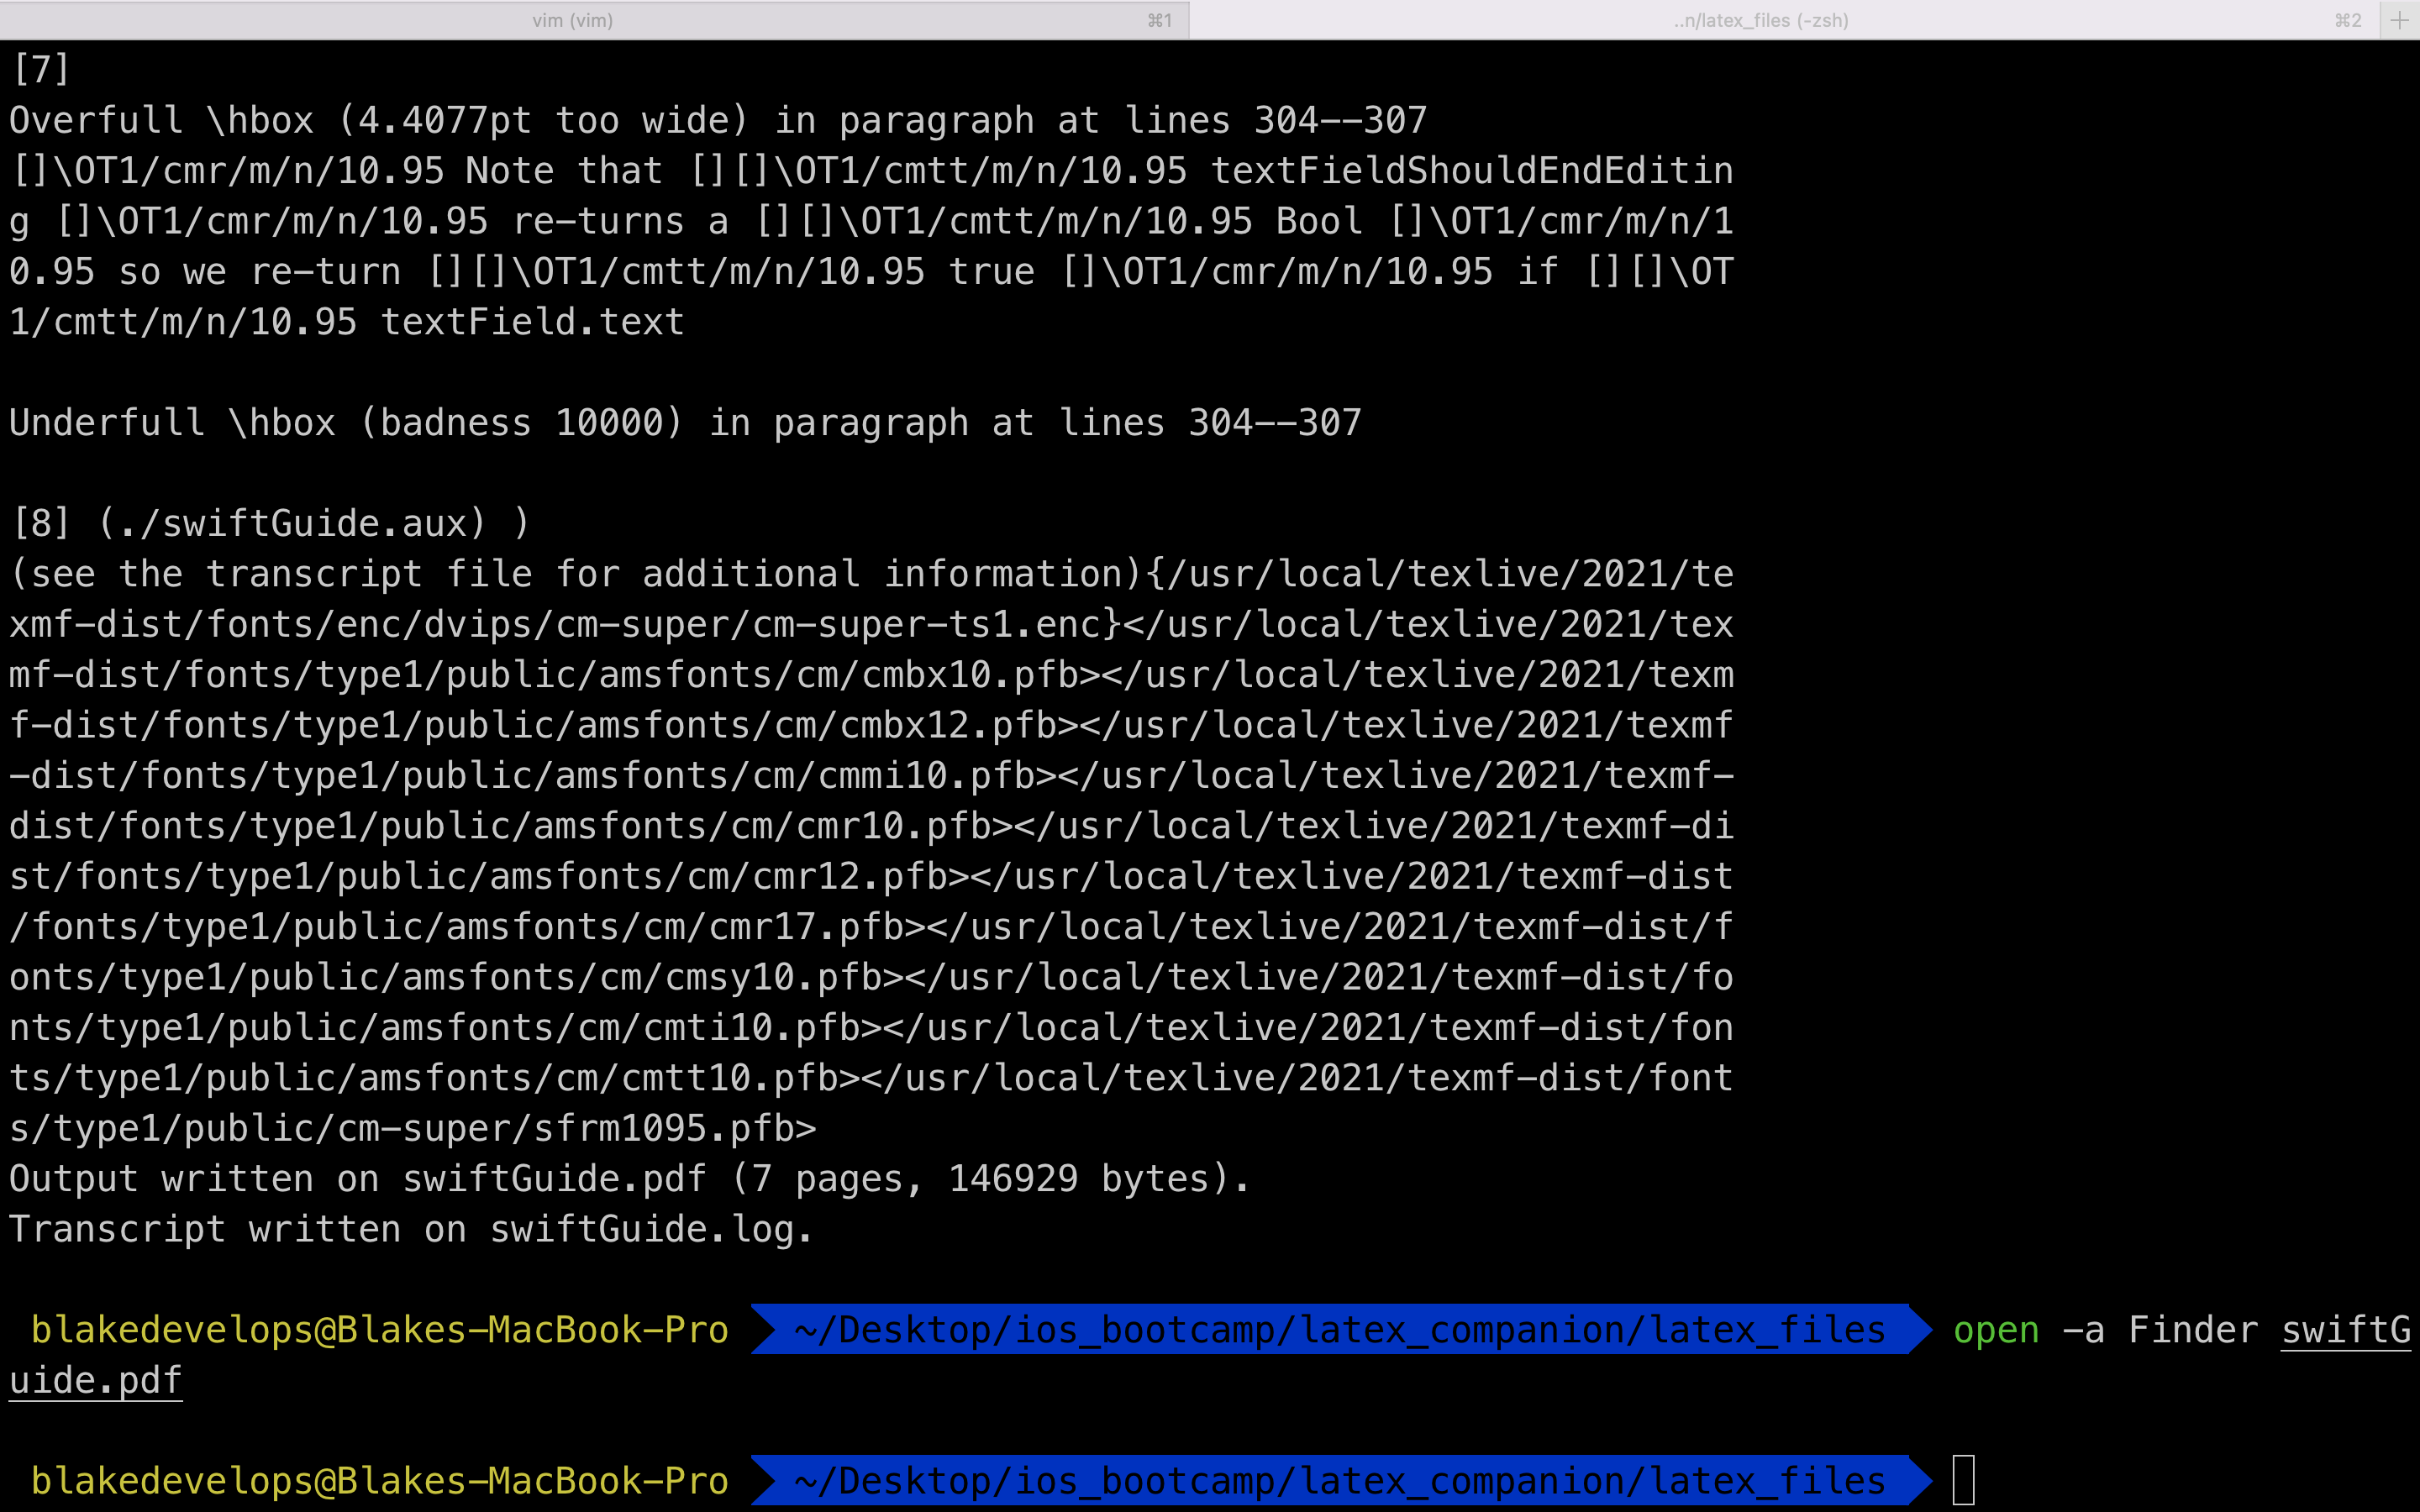
\includegraphics[scale=.12]{terminal_screenshot}
    \caption{"The powerful yet elusive Terminal."}
\end{figure}

Here's the nitty-gritty of it. You enter a command into the Terminal, and it gives you a response. But I like to imagine it
like an old school text RPG. You can move around, you can check your inventory, you can fight monsters (call functions!),
etc., etc. It's the same thing. Well, what are the commands that are available to you? \\\

\begin{enumerate}
    \itemsep0em
    \item{Move from one directory to another: \verb+cd targetDirectory+}
    \item{List the contents of the current directory: \verb+ls+}
    \item{Create a new folder in the current directory: \verb+mkdir newDirectory+}
    \item{Create a new file: \verb+touch newFile+}
    \item{Delete a file: \verb+rm fileToRemove+}
    \item{Move a file: \verb+mv fileToMove targetDirectory+}
\end{enumerate}

\begin{figure}[ht]
    \centering
        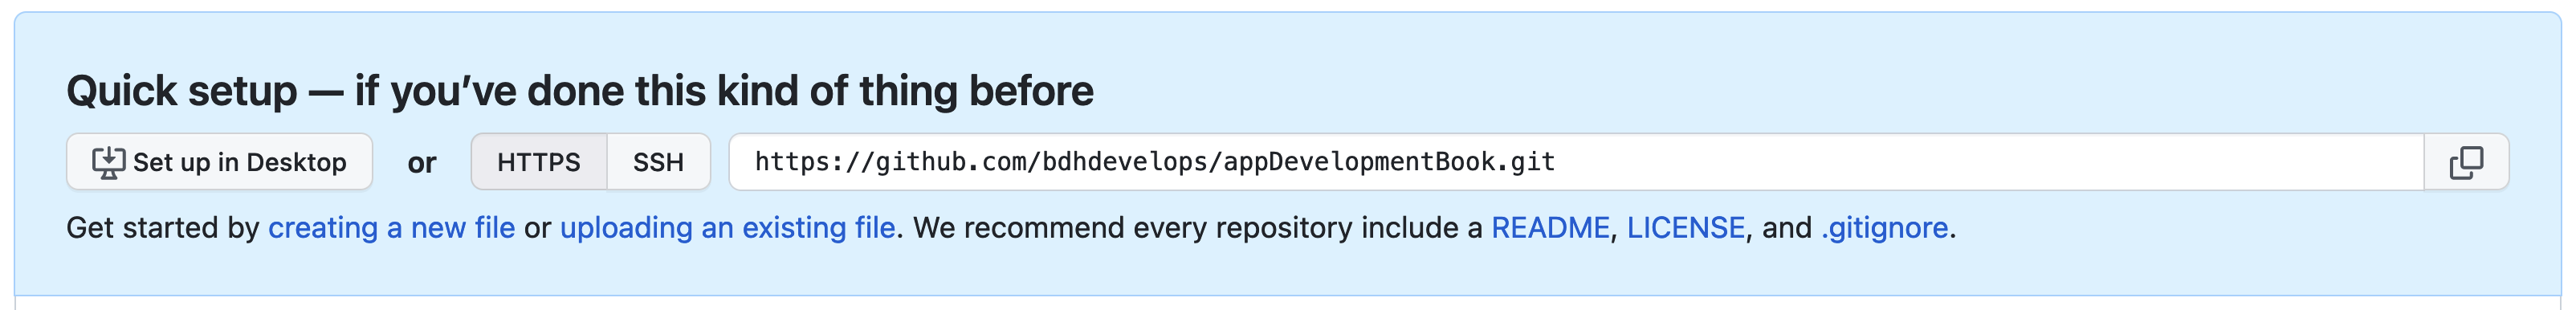
\includegraphics[scale=.3]{git_repository_URL_screenshot}
    \caption{"The URL from your new initilized GitHub repository you should copy from GitHub."}
\end{figure}

\subsection*{vim}

\subsection*{git}

\begin{enumerate}
    \itemsep0em
    \item{\verb+gh repo create+}
    \item{\verb+git init+}
    \item{\verb+git add *+}
    \item{\verb+git commit -m "Changes I've made since last push"+}
    \item{Visit GitHub and copy the source link for your repository. We will call this \verb+URL+.}
    \item{\verb+git remote add origin URL+}
    \item{\verb+git push -u origin master+}
\end{enumerate}



\subsection*{Version control}

\section{HTML and CSS}

Now that you're a pro at navigating the Terminal (or iTerm, whichever path you've chosen), we're going to get to building
apps. And we're going to jump right in by learning how to build attractive website with just HTML and CSS. A good
way to think about these two languages is like a house: HTML is the wood and beams and foundation, CSS is the paint
and decorations and all the things that make a house nice and cozy. Take a look at the HTML file below. \\

\subsection*{Basic HTML File}

\begin{figure}[ht]
\centering
\begin{BVerbatim}
index.html
-----------------------------------------------------------------------
1  <!DOCTYPE html>
2  <html>
3      <head>
4          <meta charset="utf-8">
5          <meta name="viewport" content="device-width", initial-scale="1">
6          <title> My Webpage </title>
7      </head>
8      <body>
9          <p> This is a paragraph! </p>
10     </body>
11 </html>
-----------------------------------------------------------------------
\end{BVerbatim}
\caption{Boiler plate HTML.}
\end{figure}


I'm going to tell you right now there's a heck of a lot of stuff you can ignore here. In fact, here's another copy with 
all the extra fluff hidden: \\

\begin{figure}[ht]
\centering
\begin{BVerbatim}
index.html
-----------------------------------------------------------------------
2  <html>
3      <head>
6          <title> My Webpage </title>
7      </head>
8      <body>
9          <p> This is a paragraph! </p>
10     </body>
11 </html>
-----------------------------------------------------------------------
\end{BVerbatim}
\caption{All the HTML you need to worry about right now.}
\end{figure}

Lets work inside out. The string \verb+"This is a paragraph!"+ lives inside the \verb+<p>+ element (where \verb+p+
stands for paragraph). The \verb+<p>+ element lives inside the \verb+<body>+ element. If you examine the hierarchy
of the elements, you'll see that \verb+<body>+ doesn't live in \verb+<head>+ and \verb+<head>+ doesn't live in \verb+<body>+, but 
\verb+<head>+ lives on top of \verb+<body>+. So on your webpage, the head will appear above the body. Inside the \verb+head+ element lives the 
\verb+<title>+ element. Finally, you'll see that head and body live inside the biggest element, \verb+<HTML>+. \\

CSS is very, very simple. Just like it's easier to paint a house than it is to build it, CSS is that much easier than
HTML. Let's say we want to paint the text inside the paragraph white. With code, all we need to do is have some way
to select the paragraph we want to paint, and then "paint it". Two step process. One way we can select the paragraph is
by giving it an \verb+id+. How do we do that? Simple. Alter the code for the paragraph to look like this: \\

\begin{figure}[ht]
\centering
\begin{BVerbatim}
        <p id="paragraphToPaint"> This is a paragraph! </p>
\end{BVerbatim}
\end{figure}

Now, our parapgraph has an \verb+id+ of \emph{paragraphToPaint}. Okay, now that our paragraph has a name we can point to,
we can paint it. The CSS code, again, is very simple: \\

\begin{figure}[ht]
\centering
\begin{BVerbatim}
#paragraphToPaint {
    color: white;
}
\end{BVerbatim}
\end{figure}

Here, the octothorpe (\#) means we're talking about an \verb+id+, \verb+paragraphToPaint+ is the value stored in our
\verb+id+, \verb+color+ is the selector for text color, and \verb+white+ is a premade color we're allowed to use. Here's the 
catch with \verb+ID+s. You can only use 'em once. \\

For example, if we had three paragraphs and we wanted to paint them
all white, we couldn't assign them all the \verb+id paragraphToPaint+. Instead, we use what's called a \verb+class+.
We can use as many of those as we like. The only two differences are: one, we use a \verb+.+ instead of a \verb+#+; 
and two, we use the term \verb+class+ instead of \verb+id+. Here's the code:

\begin{figure}
\centering
\begin{BVerbatim}
        <p class="paragraphsToPaint"> This is a paragraph! </p>

.paragraphToPaint {
    color: white;
}
\end{BVerbatim}
\end{figure}

This will ensure that all of the paragraph receive a fresh coat of white paint. We can assign classes and IDs to just
about any HTML element, allowing us a wide variety of avenues to take when designing an app. Additionally, CSS has a
incredible array of selectors that allow you to make a website look like anything you can dream of. It's super easy
to change background colors, fonts, borders, margins, the list goes on and on. Literally. You can find a list of
all CSS properties here (check out the bar on the left):

\begin{figure}[ht]
\centering
\begin{BVerbatim}
https://www.w3schools.com/css/default.asp
\end{BVerbatim}
\end{figure}

\section{JavaScript, HTML, CSS, and Web Development}

\section{Xcode, Swift 5, and iOS Development}

\subsection*{Section 1: Getting Started with iOS Development and Swift 5}

\subsection*{15: The I Am Rich App}

\subsubsection*{1st Module Game Plane}

Very simple app that sold for \$999. It had no functionality. Eight people bought it. \\

This module will cover the following:
\begin{enumerate}
    \itemsep0em
    \item{How to create and set up a new iOS project from scratch.}
    \item{Get an overview of Xcode, the software for creating iOS apps.}
    \item{How to design your app in Xcode using iOS components.}
    \item{How to incorporate your own image assests into your app.}
    \item{How to design and create a custom app icon.}
    \item{How to run your app on a Simulator and the iPhone.}
\end{enumerate}

\subsection*{17: Let's Create a Brand New Xcode Project}

\subsubsection*{Creating and setting up a new iOS project from scratch}

Open Xcode. Click \textbf{Create a new Xcode project}. Create an iOS $\Rightarrow$ App. 
Set \textbf{Interface} to \emph{Storyboard}. Set \textbf{Organization Identifier} to 
\emph{com.yourNameHere}. The other defaults are fine: \textbf{Team} can stay \emph{none}; Life Cycle can stay
\emph{UI Kit App Delegate}; \textbf{Language} is \emph{Swift}; and the three checkboxes at the
bottom remain unchecked. Click \textbf{Next} and save your file anywhere with any name. \\

\subsubsection*{Note! Xcode constantly saves the changes you make to your code.}

If you ever want to find out where any of your files live, you can right click on any file in the 
file tree at the top right and click \textbf{Show in Finder}. This will open a Finder window 
containing your file. You can always navigate to that folder and open the project by double-clicking
on the \emph{.project} file.

Next we will familiarize ourselves with Xcode's layout.

\subsubsection*{Getting an overview of Xcode}

Expand Xcode as much as possible and open your project. The first screen to pop up is the General tab.
We can change our minimum supported iOS version here. We can choose if we want it to run on iPhone
and iPad or just one. We can limit our app to only selected orientations/rotations. We can choose
our Status Bar style. We do most of our important work within the .swift and .storyboard files. \\

The Xcode layout is split up into four main  areas: 
\begin{enumerate}
    \itemsep0em
    \item{the \textbf{ Status Bar} at the top,} 
    \item{the \textbf{Navigator Bar} at the left,}
    \item{the \textbf{Main Storyboard} at the center (when \emph{Main.storyboard} is selected in the
        \textbf{Navigator Bar})}
    \item{the \textbf{Inspector Bar} at the right.}
\end{enumerate}

In the \textbf{Inspector Bar}, there is a tab called the \textbf{Size Inspector}. First drag and drop an
element onto the story board from the \textbf{Object Library} (plus shaped button at the upper
right of the storyboard view. Select the element. Then, at the top of the \textbf{Inspector Bar}, 
navigate to the \textbf{Size Inspector}. Here, you can set the $x$ and $y$ coordinates of the center
of the element; additionally you can set the \emph{height} and \emph{ width} properties 
of the element. \\

While a storyboard is selected, there is a bar visible just to the right of the \textbf{Navigator Bar} 
called the \textbf{Document Outline}. If this were PhotoShop, this would be where the \emph{layers}.
Finally, the very bottom pane is the \textbf{Debug Pane}.

\subsubsection*{Note! All of these bars and windows can be toggled on and off.}

Xcode has Light and Dark Mode capability -- head to  \textbf{Xcode} $\Rightarrow$ \textbf{Preferences...}
$\Rightarrow$ \textbf{Appearance} to select which one you like.

\subsection*{19: Let's Design the User Interface!}

\subsubsection*{Design your app in Xcode using iOS components}

Ensure \emph{Main.storyboard} is selected in the \textbf{Navigator Bar}. At the bottom of the storyboard
view there is a tiny icon of an iPhone next to the text``iPhone 11". By clicking on either, we can
selected which phone Xcode will emulate while running our program. Different iPhones have different
aspect ratios, resolutions, etc. and will display the same app differently. \\

In the storyboard view, if things are ever wonky, you can click on \emph{View Controller Scene} in the
\textbf{Document Outline} to bring things back to center. When dragging an object from the
\textbf{Object Library} onto the storyboard, there are guidelines for it to snap to. \\ 

Example: drag a label onto a storyboard. Navigate to \textbf{Attributes Inspector} and change the
text of the label. Change the color to white. Change the font size. We can change the \emph{background
color} of a \emph{View}.

\subsection*{Section 13: Networking, JSON Parsing, APIs, and Core Location}

\subsection*{142: What You'll Make}

A beautiful weather app that can get live weather data for the phone's GPS location or search for your own location.
The app is also Dark Mode enabled. Here are some core concepts:

\begin{enumerate}
    \itemsep0em
    \item{How to create a dark-mode enabled app and use vector assets.}
    \item{Learn to use the \emph{UITextField} to get user input.}
    \item{Learn about \textbf{Swift Protocals} and the \textbf{Delegate Design Pattern.}}
    \item{Learn to work with APIs by making HTTP requests with \emph{URLSession}.}
    \item{Parse JSON with the native JSONDecoder.}
    \item{Learn to use computed properties, closures, and extensions.}
    \item{Learn to use Core Location to get the GPS data.}
\end{enumerate}

\subsection*{143: Dark Mode and Working with Vector Assets}

\subsubsection*{Setting Up Dark Mode Capability for Our App}

As of iOS 13, Dark Mode is available to the entire operating system. An explanation on how colors work with Dark Mode.
The weather app uses SF Symbols, Apple's proprietary bundle of symbols for use in iOS development. \\

\subsection*{144: Learn to Use the UITextField}

The \emph{Text Field} object allows the user to input some data into a text field using iOS's keyboard. You can set many
properties of the UITextField in the \emph{Inspector Bar}, including one called \emph{Secure Text Entry} which obscures
the user's input (as if they were putting in a password). Additionally, one can change the value of the return key.
For example, instead of having the return key have text "return", you can have it say "go".\\

Let's set up \emph{Main.storyboard}. Create IBOutlets for the image, the temperature label, city label, and for the search
field. It should look like this when you're done.

\begin{verbatim}
WeatherViewController.swift
---------------------------

import UIKit

class WeatherViewController: UIViewController {
    @IBOutlet weak var conditionImageView: UIImageView!
    @IBOutlet weak var temperatureLabel: UILabel!
    @IBOutlet weak var cityLabel: UILabel!
    @IBOutlet weak var searchTextField: UITextField!

    override func viewDidLoad() {
        super.viewDidLoad()
    }
    // @IBActions go below me
    // ...
}
\end{verbatim}

We now wish to add an \verb+@IBAction+ below our \verb+viewDidLoad+ function by Option-dragging from the search bar to the space
between the last two curly braces. Name the \verb+@IBAction+ \verb+searchPressed+ and set the \emph{Type} to \verb+UIButton+.
The idea: user taps on the search field, types in the name of a city, presses the search button, and then we'll be able
to access \verb+searchTextField+ to see what the user typed. \\

We can access the value of the \verb+searchTextField+ using the \verb+text+ method and print it to the console:

\begin{verbatim}
    @IBAction func searchPressed(_ sender: UIButton) {
        print(searchTextField.text)
    }
\end{verbatim}

This is not to be confused with \emph{Placeholder} text, which is text that just sits in the text field until the user
interacts with it. \\

Because \verb+searchTextField.text+ has the possibility of being \verb+nil+, it is an optional type and must be unwrapped.
One way we can do this is by adding an exclamation point:

\begin{verbatim}
        print(searchTextField.text!)
\end{verbatim}

If you're using the iPhone simulator to run your apps and the keyboard is nowhere to be found, the shortcut is Command-K ti
bring it back. \\

Try running the app and typing something into the search field. Press the return button on the iOS keyboard. And... nothing
happens. We can't use an \verb+IBAction+, so we need to think of another way to get the button to do what we want it to do.
And that's by using a \verb+delegate+. \\

Start by adding a comma and \verb+UITextFieldDelegate+ after \verb+UIViewController+ in \emph{WeatherViewController.swift}:

\begin{verbatim}
class WeatherViewController: UIViewController, UITextFieldDelegate {
    ...
}
\end{verbatim}

Inside \verb+viewDidLoad()+ we are going to initialize the \verb+delegate+ as \verb+self+. 

\begin{verbatim}
        searchTextField.delegate = self
\end{verbatim}

When the interacts with \verb+searchTextField+, the search field will notify \verb+WeatherViewController+ about what happened.
For example, we are going to use the premade function \newline \verb+textFieldShouldReturn+ which asks the delegate
(the weather view controller) if the text field should process the pressing of the return button. \\

The code in the following function executes exactly when the return button is pressed on the keyboard.

\begin{verbatim}
    func textFieldShouldReturn(_ textField: UITextField) -> Bool {
        print(searchField.text!)
        return true
    }
\end{verbatim}

One problem. The keyboard won't dismiss itself after the return key is pressed. We can resolve this by using the 
\verb+endEditing+ method. We're going to add it to both \verb+searchPressed+ and \verb+textFieldShouldReturn+:

\begin{verbatim}
    @IBAction func searchPressed(_ sender: UIButton) {
        searchTextField.endEditing(true)
        print(searchTextField.text!)
    }

    func textFieldShouldReturn(_ textField: UITextField) -> Bool {
        searchTextField.endEditing(true)
        print(searchTextField.text!)
        return true
    }
\end{verbatim}

Now the keyboard should disappear upon either a press of the search button or of the return key on the keyboard. We
now want to clear the search field after we're done editing it. Again, there's a \verb+delegate+ method for that. \\

\begin{verbatim}
    func textFieldDidEndEditing(_ textField: UITextField) {
        searchTextField.text = ""
    }
\end{verbatim}

This code will run any time a text field is done being editing, as long as the \verb+endEditing+ method is included in the
function. Finally, we have \verb+textFieldShouldEndEditing+, where we can define functionality for when the user tries
to get out of the keyboard screen. Under what circumstances might we want to lock a user into the keyboard screen?
Well, we can check to make sure that the user is inputting what we want them to. \\

Think of when you sign up for a new website and we want to lock the user into the keyboard screen until the input a 
password that has a number, an uppercase character, and a special character. Below we make sure that 
\verb+textField.text+ isn't an empty string or else we use the text field's \emph{placeholder} value 
to display a message to the user:

\begin{verbatim}
func textFieldShouldEndEditing(_ textField: UITextField) -> Bool {
    if textField.text != "" {
        return true
    } else {
        textField.placeholder = "Type something..."
        return false
    }
}
\end{verbatim}

Note that \verb+textFieldShouldEndEditing+ returns a \verb+Bool+ so we return \verb+true+ if 
\newline \verb+textField.text+ is not an empty string (and therefore the user entered something, so yes, 
the text Field Should End Editing). And we return \verb+false+ in the other case and keep the user just where they are. \\

Finally, we wish to access whatever text the user inputted into the search field so that we can use it to search for
weather. We're going to utilize our \newline \verb+textFieldDidEndEditing+ for this (which again, triggers when the user exits
the keyboard screen).

\begin{verbatim}
func textFieldDidEndEditing(_ textField: UITextField) {
    // Use searchTextField.text to get the weather for the city.
    searchTextField.text = ""
}
\end{verbatim}


\subsubsection*{145 Swift Protocals}

What is a Swift Protocol and what does it allow us to do? Think of it as a certification in your resume. Imagine a 
CPR certification: doctors need it, paramedics need it, etc. A protocol defines a set of requirements. Then, a 
class or struct adopts a protocol and from there on it needs to meet the requirements set forth in the protocol:

\begin{verbatim}
protocol MyProtocol {
    // Define requirements.
}

struct MyStruct: MyProtocol {}
ckass MyClass: MyProtocol {}
\end{verbatim}

Create a new \textbf{macOS} $\Rightarrow$ \textbf{Command Line Tool} in Xcode and name it Protocols Demo, hit Finish,
and save it anywhere. Clear out \emph{main.swft}. Let's define a class for birds. For now, our bird can fly and lay
an egg if it's female. Additionally, let's create an Eagle class from our Bird class, but let's say eagles can Soar
in addition to Fly. Finally, we'll create a Penguin class, and we'll say Penguins can swim too.

\begin{verbatim}
main.swift
--------------------------------------------------------------------------------
1  class Bird {
2      var isFemale = true
3      func layEgg() {
4          if isFemale() {
5              print("The bird lays an egg.")
6          }
7      }
8      func fly() {
9          print("The bird flies.")
10      }
11  }
12
13  class Eagle: Bird {
14      func soar() {
15          print("The eagle soars.")
16      }
17
18  class Penguin: Bird {
19      func swim() {
20          print("The penguin swims.")
21  }
--------------------------------------------------------------------------------
\end{verbatim}

Alls well and good here. Our birds and eagles can fly, lay eggs, soar. Neato. But what's the issue? Well, what about 
penguins? Penguins can swim and lay eggs, but they can't fly or soar. We'd like to create a Penguin class from our Bird
class, but we can't have our penguins be flying around. Let's say we have a museum and they want to demonstrate 
the flying capabilities of different birds. \\

We'll create a struct for the museum and it will have a method 
\verb+flyingDemo+ that takes as input only objects that can fly (here, birds). Next, we'll instantiate an Eagle object
and have our Mueseum demonstrate it's flying capabilities.

\begin{verbatim}
struct Museum(flyingObject: Bird) {
    func flyingDemo(flyingObject: Bird) {
        flyingObject.fly()
    }
}

myEagle = Eagle()
Museum.flyingDemo(flyingObject: myEagle)
\end{verbatim}

Run the program, and the console should log \verb+"The bird flies."+ Remember, this works because the Eagle class
inherited the \verb+fly+ method from the \verb+Bird+ class. Now, if we made a Penguin object and passed it to
tbe Museum's \verb+flyingDemo+ method, we'd get the same results. But penguins can't fly! We'll deal with that later. \\

Let's say our museum wants to demonstrate other types of flight, like airplanes and helicopters. We could create
classes for these inherting from \verb+Bird+ and override the \verb+fly+ method, but then our airplanes and helocp[ters
would be able to lay eggs too. Rather, we want museum to be able to check if an object can fly irregardless if it's
a bird or not, then demonstrate it's flying capabilities. We do this by using \verb+protocols+. \\

We'll create a \verb+protocol CanFly+ at the beginning of our \emph{main.swift}. Next, we'll define the fly requirement by using
the header of a function definition (not the body of the function!). Next, we assign the \verb+protocol+ to all classes
that can fly by adding ``\verb+, CanFly+'' after our class names. Finally, we ensure each class marked with the 
\verb+protocol+ actually has a \verb+fly+ method. If you mark a class with \verb+CanFly+ and don't give it \verb+f;y+
method, you will get an error! Note that we don't mark penguin, because penguins can't fly darnit! \\

\begin{verbatim}
main.swift
--------------------------------------------------------------------------------
0  protocol CanFly {
1       func fly()
2       // Notice how we're not defining any fly function right here
3  }
4
5  class Bird {
6       var isFemale = true
7       func layEgg() {
8           print("The bird lays an egg.")
9       }
10 }
11 
12 class Eagle, CanFly {
13      func fly() {
14          print("The eagle flies.")
15      }
16      func soar() {
17          print("The eagle soars.")
18      }
19 }
20
21 class Penginuin {
22      func swim() {
23          print("The penguin swims.")
22      }
25 }
26
27 class Airplane {
28      func fly() {
29          print("The airplane flies.")
30      }
31 }
--------------------------------------------------------------------------------
\end{verbatim}

Finally, we can refactor our \verb+Museum+ struct definition so that it only accepts objects with a \verb+fly+ methods
by using our \verb+CanFly protocol+ as the datatype:

\begin{verbatim}
struct Museum {
    func FlyingDemo(flyingObject: CanFly) {
        flyingObject.fly()
    }
}
\end{verbatim}

Note that you can define and use multiple \verb+protocols+ defining your class our struct like so:
\verb+class MyClass: ClassToInheritFrom, FirstProtocol, SecondProtocol, ...+ and etc.

\subsubsection*{AJAX and API's in JavaScript}

In this section, we're going to learn how to make requests using JavaScript code. It's a concept called \textbf{AJAX}:
making requests behind the scenes will the user is interacting with the web app. \textbf{AJAC} stands for Asynchronous
JavaScript and XML (even though instead of XML we use JSON).
For example, if we're scrolling down 
Reddit we want the app to continuously offer new posts. Or, if we have a search bar and we want to present live
search results as the user types. \\

When you use a browser to navigate to a website, you are a making a request. Usually, this request returns a mess of HTML
which your browser then constructs into a website you can use. With \textbf{AJAX}, we want to request a stripped down
object filled with information that we can manupulate easily. The name of this type of object is \textbf{JSON}. Here's an example 
of a request you can make that will return one of these stripped down objects: \\

\centerline{api.cryptonator.com/api/ticker/btc-usd}

If you follow this link your browser will return an object like the followng: \\

\begin{mdframed}[hidealllines=true,backgroundcolor=codeBackgroundColor]
    {\color{punctuationColor} \tt 
{    {\fontfamily{DejaVuSansMono}
    \centerline{api.cryptonator.com/api/ticker/btc-used in your browser} 
    \centerline{\rule{7in}{1.5pt}}   
    \vspace{.5cm}
1         \{ \\
2             \phantom{xxxxx}{\bf \colorobject{"ticker"}}: \{ \\
3             \phantom{xxxxxxxxxx}{\it {\color{variableNameColor}"base"}}: {\color{stringColor}"BTC"}, \\
4             \phantom{xxxxxxxxxx}{\it \color{variableNameColor}{"target"}}: {\color{stringColor}"USD"}, \\
5             \phantom{xxxxxxxxxx}{\it \color{variableNameColor}{"price"}}: {\color{stringColor}"46318.38591953",} \\
6             \phantom{xxxxxxxxxx}{\it \color{variableNameColor}{"volume"}}: {\color{stringColor}"16442.72301906"}, \\
7             \phantom{xxxxxxxxxx}{\it \color{variableNameColor}{"change"}}: {\color{stringColor}"249.44780355"} \\
8             \phantom{xxxxx}\}, \\
9             \phantom{xxxxx}{\it \color{variableNameColor}{"timestamp"}}: {\color{stringColor}1641249902}, \\
10            \phantom{xxxxx}{\it \color{variableNameColor}{"success"}}: {\color{trueBoolColor}true}, \\
11            \phantom{xxxxx}{\it \color{variableNameColor}{"error"}}: {\color{stringColor}""} \\
12         \}
    }
    }}
\end{mdframed}

An \textbf{API} is an application programming interfrace; these are portals into other applications that allow us to
gather information, etc. A lot of more useful APIs cost money to use. Lots of APIs work with a data format called 
\textbf{JSON}, or JavaScript Object Notation. We like to use it because it is uniform and universal. It looks like
a JavaScript object, but with a few key differences. Each key must by surrounded by quotes in the definition. \\

The types of data a JSON object can hold include: objects, arrays, strings, numbers, booleans, and null.
Now, when we first get our JSON object, it's just a string. It needs to be parsed into a JavaSCript object. Luckily
there's an easy JavaScript funciton for that: \verb+JSON.parse+. For now, let's save a dummy JSON object in a variable,
then call our parse method on it:

\begin{verbatim}
const data = "{"key1":value1,"key2":value2,"key3":value3}"
const parsedData = JSON.parse(data)
\end{verbatim}

Now we can access \verb+value1+, \verb+value2+, \verb+value3+ with \verb+parsedData.key1+, \verb+parsedData.key2+, etc.
etc. Additionally, we can go the other way. We can turn a JavaScript object into a string for API usage:
\verb+JSON.string+. \\ 

\subsubsection*{Working with Postman}

The most basic thing to do with Postman: enter a URL and press Send. If the URL is a webpage, it will return HTML. If it's
and API link, it will return a JSON object. There are many different types of requests that can be made, but for now
we'll be using the \textbf{GET} request, veruses the \textbf{POST} reqhest, which will send some to the server. \\

A JSON object consists of a few different parts: the body (which contains the code we've been working with above),
the status (which provides information about the success or failure of our request), and headers (key/value pairs
that provide additional information about the object like a timestamp, content-type, etc.). 

\subsubsection*{Query Strings and Headers}

Example: tmaze.com/api. Query string: 

\begin{verbatim}
/search/shows?q=:query 
http://api.tvmaze.com/search/shows?q=girls
\end{verbatim}

TVMaze will return multiple results in a JSON object if there are multiple matches. Show lookup endpoint:

\begin{verbatim}
/lookup/shows?imdb=:imdbid
http://api.tvmaze.com/lookup/shows?imdb=tt0944947
\end{verbatim}

Query strings are information we can append to URLs that will impact what the API returns. \\

Episode by TVMaze id, season and number. Demonstrate how we can pass multiple values through the URL:

\begin{verbatim}
/shows/:id/episodebynumber?season=:season&number=:number
http://api.tvmaze.com/shows/1/episodebynumber?season=1&number=1
\end{verbatim}

We can use Postman to build query string URLs. \\

Openweathermap API. You can pass in a city, or a latitude and longitute. \\

Icanhazdadjoke. Demonstrating how to give a header to an API that requires it. In Postman, enter 
https://icanhazdadjoke.com into the bar. Next, click the Headers tab and add key \verb+Accept+ with 
value \verb+application/json+. Pressing Send, and we'll get a JSON object with an \verb+id+, a random joke,
and a status. 

\subsubsection*{Making XHR's, or XMLHttpRequests}

Horrible, old way to do this. Just for appreciation of newer methods. First we make an XMLttoRequest object.
Next we define \verb+onload+ and \verb+onerror+ callbacks. Then we open the request, then we send the request. Example:

{\small
\begin{verbatim}
app.js
--------------------------------------------------------------------------------
const req = new XMLHttpRequest();
req,onload = function() {
   console.log("Request succeeded.");
   console.log(this);
}
req.onerror = function() {
   console.log("Request failed.");
   console.log(this);
}

req.open('GET', 'https://api.cryptonator.com/api/ticker/btc-usd');
req.send();
--------------------------------------------------------------------------------
\end{verbatim}
}

We receive back a request object with a \verb+responseText+  property that includes the data we wish to parse. We'll save
it as a variable \verb+data+ in our \verb+onload+ function and log the ticker price:

{\small
    \begin{verbatim}
        const data = JSON.parse(this.responseText);
        console.log(data.ticker.price);
    \end{verbatim}
}

That's all for XMLHttpRequests.

\subsubsection{The Fetch API}

Written is response to how sucky XMLHttpRequests are. Fetch does the same thing, but it uses promises, async, and
await. Here's the syntax; the result is a Promise.

{\small
    \begin{verbatim}
        fetch('https://api.cryptonator.com/api/ticker/btc-usd')
            .then(res =>
                console.log("RESPONSE:", res);
            })
            .catch((e => {
                console.log("ERROR:", e);
            })
    \end{verbatim}
}

Fetch's \verb+Promise+ result will resolve as soon as it has received the object's headers. So, inside \verb+.then+,
there is still a possibility the request will fail. We will add the function \verb+res.json()+ which returns 
a \verb+Promise+ that resolves when all of the JSON object is loaded. We'll then return \verb+res.json()+ and chain
another \verb+.then+ which will run once \verb+res.json+ has resolved:

\begin{verbatim}
            .then(res => {
                console.log("Waiting for JSON object parson to finish."
                return res.json()
            })
            .then(data => {
                console.log("Data parsed:", data);
                console.log(data.ticker.price);
            })
\end{verbatim}

And now using \verb+async+ with error handling:

{\small
\begin{verbatim}
const fetBitCoinPrice = async () => {
    try {
        const res = await fetch('https://api.cryptonator.com/api/ticker/btc-usd');
        const data = await res.json();
        console.log(data.ticker.price);
     catch (e) {
        console.log("Something went wrong.")
     }
}
\end{verbatim}
}

\subsubsection*{Intro to Axios: A Library for Making HTTP Requests}

Axios is a JavaScript library which must be included in our HTML in order for it to work:

{\small
\begin{verbatim}
<script src="https://cdn.jsdelivr.net/npm/axios/dist/axios.min.js">
</script>
\end{verbatim}
}

{\small
\begin{verbatim}
app.js
--------------------------------------------------------------------------------
axios.get('https://api.cryptonator.com/api/ticker/btc-usd')
    .then(res => {
        console.log(res.data.ticker.price);
    })
    .catch(err => {
        console.log("Error:", err);
    })

const fetchBitcoinPrice = async () => {
    try {
        const res = 
            await axios.get('https://api.cryptonator.com/api/ticker/btc-usd')
            console.log(res.data.ticker.price);
    } catch (e) {
        console.log("Error: ", e);
    }
\end{verbatim}
}

Returns a Promise containing data that's already been parsed! \verb+axios.get+ only resolves once the entire JSON
object has been downloaded, unlike \verb+fetch+ which resolves after the headers has been received. Next we'll learn
how to configure headers using axios. \\

\begin{verbatim}
const getDadJoke = async () => {
    const config = { headers: { Accept: 'application/json' } };
    const res = await axios.get('https://icanhazdadjokes', config);
    console.log(res.data.joke);
}
\end{verbatim}

\section{References}

\subsubsection*{Syntax Highlight}

\end{document}
